\chapter{Brugermanual}

Det første der møder en når man starter spillet er skærmbilledet der ses på figur \ref{fig:startup}. Den blinkende tekst under logoet angiver at brugeren skal trykke på en valgfri tast for at starte spillet. ASCII arten af rattet skulle gerne give en indikation af hvordan spillet styres. Et billede af rattet til sammenligning kan ses i figur \ref{fig:rat_med_controls}.

\begin{figure}[ht]
\begin{minipage}[b]{0.5\linewidth}
\centering
\includegraphics[width=\textwidth]{figs/screenshots/startup_crop.png}
\caption{Screenshot af startup skærmen}
\label{fig:startup}
\end{minipage}
\hspace{0.5cm}
\begin{minipage}[b]{0.5\linewidth}
\centering
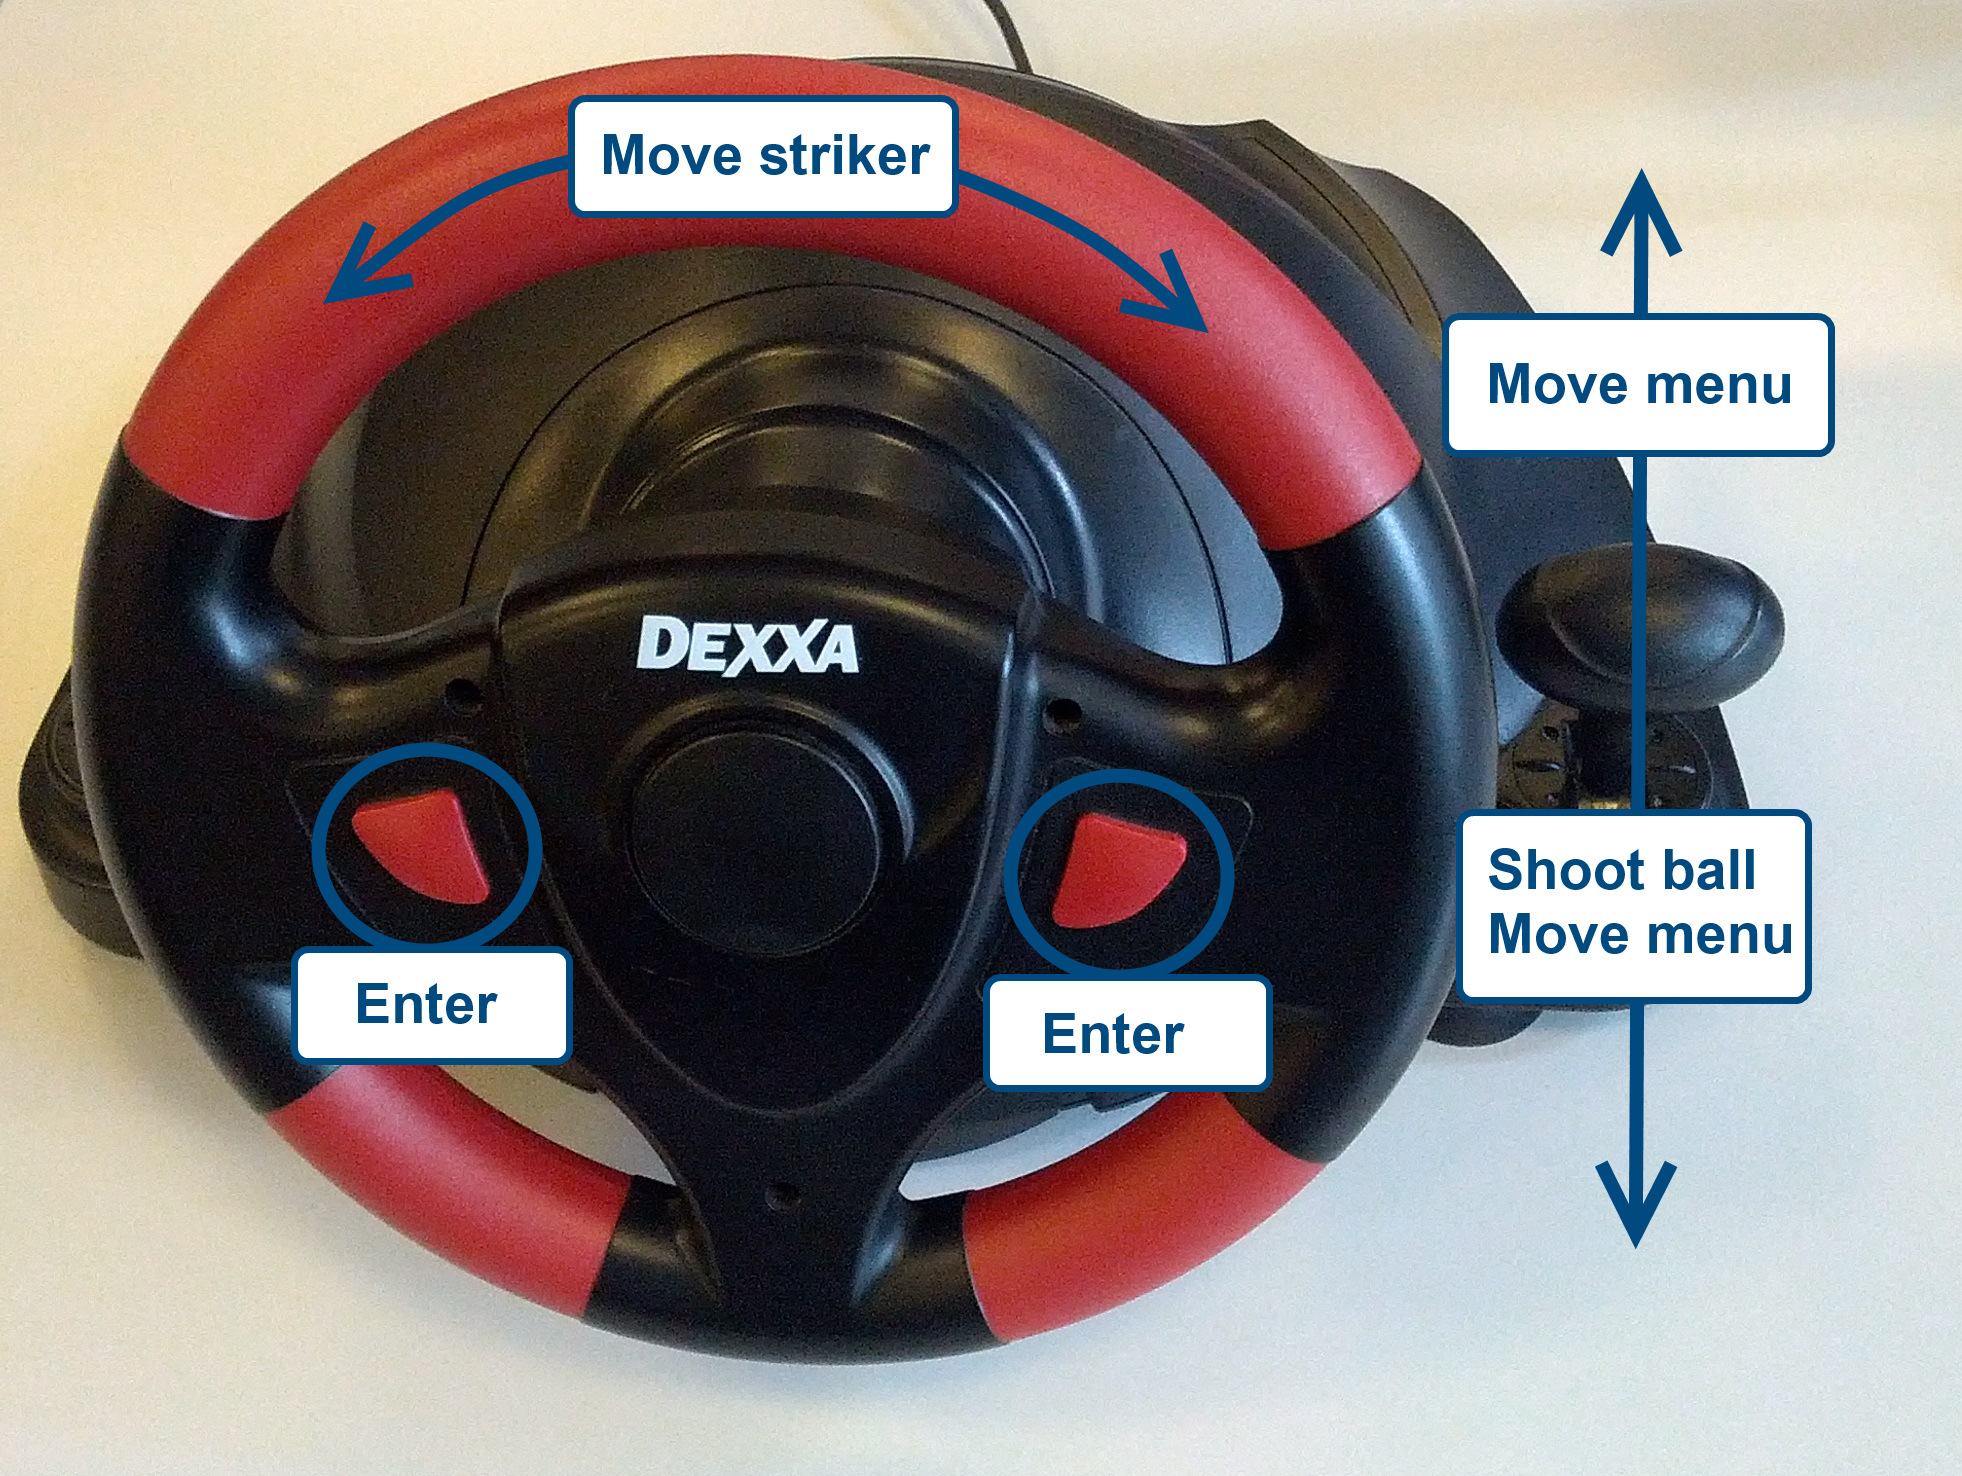
\includegraphics[width=\textwidth]{figs/rat_med_controls.png}
\caption{Oversigt over hvordan rattet bruges}
\label{fig:rat_med_controls}
\end{minipage}
\end{figure}




\begin{figure}[h!]
\centering
\includegraphics[scale=0.25]{figs/screenshots/menu_crop.png}
\caption{Screenshot af menuen}
\label{fig:menu_2}
\end{figure}



\begin{figure}[h!]
\centering
\includegraphics[scale=0.25]{figs/screenshots/gameover_crop.png}
\caption{Eksempel på screenshot game over tekst}
\label{fig:gameover_2}
\end{figure}



\begin{figure}[ht]
\begin{minipage}[b]{0.5\linewidth}
\centering
\includegraphics[width=\textwidth]{figs/screenshots/won_normal.png}
\caption{Screenshot ved gennemførsel af spillet}
\label{fig:won_normal_2}
\end{minipage}
\hspace{0.5cm}
\begin{minipage}[b]{0.5\linewidth}
\centering
\includegraphics[width=\textwidth]{figs/screenshots/won_chuck_crop.png}
\caption{Screenshot ved gennemførsel af spillet i Chuck Norris mode}
\label{fig:won_chuck}
\end{minipage}
\end{figure}












\begin{figure}[ht]
\begin{minipage}[b]{0.5\linewidth}
\centering
\includegraphics[width=\textwidth]{figs/screenshots/level1.png}
\caption{Level 1}
\label{fig:level1_2}
\end{minipage}
\hspace{0.5cm}
\begin{minipage}[b]{0.5\linewidth}
\centering
\includegraphics[width=\textwidth]{figs/screenshots/level2.png}
\caption{Level 2}
\label{fig:level2}
\end{minipage}
\end{figure}

\begin{figure}[ht]
\begin{minipage}[b]{0.5\linewidth}
\centering
\includegraphics[width=\textwidth]{figs/screenshots/level3.png}
\caption{Level 3}
\label{fig:level3}
\end{minipage}
\hspace{0.5cm}
\begin{minipage}[b]{0.5\linewidth}
\centering
\includegraphics[width=\textwidth]{figs/screenshots/level4.png}
\caption{Level 4}
\label{fig:level4}
\end{minipage}
\end{figure}

\begin{figure}[ht]
\begin{minipage}[b]{0.5\linewidth}
\centering
\includegraphics[width=\textwidth]{figs/screenshots/level5.png}
\caption{Level 5}
\label{fig:level5}
\end{minipage}
\hspace{0.5cm}
\begin{minipage}[b]{0.5\linewidth}
\centering
\includegraphics[width=\textwidth]{figs/screenshots/level6.png}
\caption{Level 6}
\label{fig:level6}
\end{minipage}
\end{figure}

\newpage